\title{MTech}
\author{Ajoy Karmakar}
\date{September 2024}
\documentclass[12pt,a4paper]{report}%Defines the document class as a report, suitable for longer documents with chapters. can write {report} instead of {article} or {book}
\usepackage[a4paper, left=2.5cm, right=2.5cm, top=2.5cm, bottom=2.5cm]{geometry}%Sets the page size to A4 and defines the page margins (2.5 cm on all sides).
\setlength{\parindent}{1em} % This controls the paragraph indent size(1em here)
\usepackage{graphicx}%Enables the inclusion of images and graphics in the document.
\usepackage{setspace}%Provides commands for setting line spacing (e.g., single or double spacing).
\usepackage{tocloft}%: Customizes the Table of Contents, allowing for changes in its layout and appearance.
\usepackage{amsmath}% Provides advanced mathematical symbols and formatting.
\usepackage{multicol}%Enables multi-column formatting, useful for newspapers or other multi-column layouts.
\usepackage{ragged2e}%Provides text alignment commands like \justify (justifies text to both margins).
%\usepackage{tabto}%for tab otherwise use vspace 1 cm
\graphicspath{ {figures/} }
\usepackage{array}
\usepackage[printonlyused,withpage]{acronym}%For Acronym NDVI Normalized Difference Vegetation Index
\usepackage{glossaries} %for glossary

\usepackage{hyperref}%Adds clickable links within the document. It also allows customization of link colors using the \hypersetup command.
\usepackage{color}%allows the use of colors in the document (in text and links).
\hypersetup{
    colorlinks=False,  % Enable-Disable colored links
    linktoc=all,      % Enable links for sections and subsections
    linkcolor=blue,   % Colour for section links
    citecolor=blue,  % Colour for citation links (set to black)
}
\renewcommand{\cftsecleader}{\cftdotfill{\cftdotsep}}%Modifies the Table of Contents dots (the leaders).
\renewcommand{\contentsname}{Table of Contents}
%\usepackage[autostyle]{csquotes} %will help for sorting in Bibliography (May be/showing error that's why muted)
\usepackage[backend=biber,style=apa,sorting=nyt]{biblatex} % Adds bibliography management using the APA style. backend=biber specifies that biber is the backend processor, while sorting=nyt sorts by name, year, title.
%\usepackage[backend=biber,style=ieee,sorting=none]{biblatex} % IEEE style Bibliography
%\parencite{} for parenthetical citations with the help of biblatex
%\textcite{} for inline citations (author-year style) with the help of biblatex
%\footcite{} for citations in footnotes, and many more with the help of biblatex
\addbibresource{mybib.bib} % adding Bibliography

\usepackage{blindtext} %for example, %Faltu Text

\usepackage{amsmath}%Used for advanced math typesetting, providing additional environments and features like equation alignment and more.
\usepackage{amssymb}%Provides additional mathematical symbols such as \mathbb{R} for real numbers and \mathbb{N} for natural numbers.
\usepackage{graphicx}%Used for including and resizing images within the document.
\usepackage{caption}%Allows customization of captions for figures, tables, and other objects in the document.
%\usepackage{natbib}%Handles bibliographies and citations with support for numeric and author-year citation styles.%Not using as I am using bib
\usepackage{geometry}%Customizes the page layout, such as margins, paper size, etc.
\usepackage{enumitem}%Customizes itemized, enumerated, and description lists, offering greater control over their appearance.
\usepackage[toc]{appendix}%Manages appendices and can include them in the table of contents.
\usepackage{cleveref}%Provides intelligent cross-referencing, so you don’t have to manually write “Figure,” “Table,” etc., every time you refer to a figure, table, or section.
\usepackage{lipsum}%Generates placeholder text (like "Lorem Ipsum") for filling out documents when you need filler text.
%%%%%%%%%%%%%%%%%%%%%%%%%%%%%%%%%%%%%%%%%%%%%%%%%%%%%%%%%%%%%%%%%%%%%%%%%%%%%%%%%%%%%%%%%%%%%%%%%%%%%%%%%%
% Title page
\begin{document}
\begin{titlepage}
   \centering
   \LARGE
    \textbf{
IMPACT OF FIRE ON CARBON FLUX IN NORTH-WESTERN HIMALAYA
}
    
    \vspace{1cm}
    \normalsize \textmd{
    Thesis submitted to Andhra University, Visakhapatnam for partial fulfilment of\\ the requirements for the award of the degree of Master of Technology \\in
    Remote Sensing and Geographic Information System\\
}
\vspace{10 mm}
 
\centering

\includegraphics[width=0.25\linewidth]{photos/Andhra_University_logo.png}
    %\caption{Enter Caption}
    %\label{fig:enter-label}
\vspace{5 mm}

\large
\textit{Submitted by}\\
\Large
    \textbf{Ajoy Karmakar}\\
    \vspace{1cm}
\large
    \textit{Supervisor}\\
\Large
    \textbf{Dr. Taibanganba Watham}\\
\vspace{0 mm}

\large
\centering
Scientist/Engineer - ‘SE’\\
Forestry and Ecology Department\\
Indian Institute of Remote Sensing, Dehradun
\vspace{ 10 mm}\\

    
\includegraphics[width=0.2\textwidth]{photos/isro_logo.png}\\
    \vspace{2mm}
    \Large
    \textbf{Indian Institute of Remote Sensing}\\
    Indian Space Research Organisation\\
    Department of Space, Government of India\\
    Dehradun – 248001\\
    \vspace{4 mm}
    May 2025
    \normalsize
\end{titlepage}
%%%%%%%%%%%%%%%%%%%%%%%%%%%%%%%%%%%%%%%%%%%%%%%%%%%%%%%%%%%%%%%%%%%%%%%%%%%%%%%%%%%%%%%%%%%%%%%%%%%%%%%%%%
%Preface
\newpage
\thispagestyle{empty} % No page number or header/footer
\null % Ensures the page starts without any additional content
\vspace{5cm} % Creates vertical space for centering the content

% Dedication content
\begin{center}
    \Large{\textsl{“As far as the laws of mathematics refer to reality,\\ they are not certain; as far as they are certain,\\ they do not refer to reality.”}}\\[1em]
    \normalsize{--- Albert Einstein}
\end{center}

\normalsize

%%%%%%%%%%%%%%%%%%%%%%%%%%%%%%%%%%%%%%%%%%%%%%%%%%%%%%%%%%%%%%%%%%%%%%%%%%%%%%%%%%%%%%%%%%%%%%%%%%%%%%%%%%
% Disclaimer Page
\newpage
\thispagestyle{empty}
\null 
\vspace{185 mm}
\section*{\centering Disclaimer}
\vspace{0.5cm}

This document describes the work carried out in partial fulfilment of the requirements for the award of the degree of Master of Technology in Remote Sensing and Geographic Information System by Andhra University, Visakhapatnam. The work is carried out at Indian Institute of Remote Sensing, ISRO, Dehradun. All views and opinions expressed therein remain the sole responsibility of the author and do not necessarily represent those of the Institute.

%%%%%%%%%%%%%%%%%%%%%%%%%%%%%%%%%%%%%%%%%%%%%%%%%%%%%%%%%%%%%%%%%%%%%%%%%%%%%%%%%%%%%%%%%%%%%%%%%%%%%%%%%%

% Declaration Page
\newpage
\thispagestyle{empty}
\section*{\centering Declaration}
\vspace{0.5cm}
\justifying{I hereby declare that the work presented in this M.Tech. thesis entitled \textbf{\textsl{“Impact of Fire on Carbon Flux in North-Western Himalaya”}} has been carried out by me and further declare that it has not been submitted earlier in part or in whole to any University or Institution for the award of any Degree or Diploma. The work embodied in this thesis has been carried out at Indian Institute of Remote Sensing (IIRS), ISRO, Dehradun under the supervision of \textbf{Dr. Taibanganba Watham, Scientist/Engineer-‘SE’, Forestry and Ecology Department, IIRS}. The extent of information derived from the existing literature has been indicated in the body of the thesis at appropriate places giving the source of information.}

\vspace{1.5cm}
\flushleft
Date:  \\
\text Place: Dehradun, India   \hfill \textbf{Ajoy Karmakar}
%%%%%%%%%%%%%%%%%%%%%%%%%%%%%%%%%%%%%%%%%%%%%%%%%%%%%%%%%%%%%%%%%%%%%%%%%%%%%%%%%%%%%%%%%%%%%%%%%%%%%%%%%%

% Certificate Page
\newpage
\thispagestyle{empty}
\section*{\centering Certificate}
\vspace{0.5cm}
\justifying{This is to certify that the work reported in this thesis entitled \textbf{\textsl{“Impact of Fire on Carbon Flux in North-Western Himalaya”}} has been carried out by \textbf{Mr. Ajoy Karmakar} in partial fulfilment of the requirement for the award of the degree of \textbf{Master of Technology (M.Tech.)} in \textbf{Remote Sensing and Geographic Information System} with specialisation in \textbf{Forest Resources \& Ecosystem Analysis} (2023-2025 batch). The work has been carried out in Forestry and Ecology Department (FED) of Indian Institute of Remote Sensing (IIRS), Indian Space Research Organisation (ISRO), Dehradun under the guidance of Dr. Taibanganba Watham.}
\vspace{2cm}

\begin{multicols}{2}
\centering \hrule \par
\vspace{0.5em}
\textbf{Dr. Taibanganba Watham}\par
\textbf{Supervisor}\par
Scientist/Engineer - ‘SE’\par
Forestry and Ecology Department\par
IIRS, Dehradun\par
\vspace{2em}
\centering \hrule \par
\vspace{0.5em}
\textbf{Dr. Hitendra Padalia}\par
Scientist/Engineer - ‘SG’ \& Head,\par
Forestry and Ecology Department\par
IIRS, Dehradun\par
\vspace{2em}
\end{multicols}

\vspace{2cm}

\begin{multicols}{2}
\centering \hrule \par
\vspace{0.5em}
\textbf{Dr. Suresh Kumar}\par
Group Director\par
\centering Agriculture, Forestry and Ecology Group\par
IIRS, Dehradun\par
\vspace{2em}
\centering \hrule \par
\vspace{0.5em}
\textbf{Dr. Pramod Kumar}\par
Dean (Academics)\par
IIRS, Dehradun\par
\vspace{2em}
\end{multicols}
%%%%%%%%%%%%%%%%%%%%%%%%%%%%%%%%%%%%%%%%%%%%%%%%%%%%%%%%%%%%%%%%%%%%%%%%%%%%%%%%%%%%%%%%%%%%%%%%%%%%%%%%%%
%ACKNOWLEDGEMENTS
\newpage
\pagenumbering{roman}
\section*{\centering Acknowledgments}
\vspace{0.5 cm}

\noindent
{\blindtext}


%%%%%%%%%%%%%%%%%%%%%%%%%%%%%%%%%%%%%%%%%%%%%%%%%%%%%%%%%%%%%%%%%%%%%%%%%%%%%%%%%%%%%%%%%%%%%%%%%%%%%%%%%%

% Table of Contents
\newpage
%\section*{\centering TABLE OF CONTENT}
\centering\tableofcontents
%%%%%%%%%%%%%%%%%%%%%%%%%%%%%%%%%%%%%%%%%%%%%%%%%%%%%%%%%%%%%%%%%%%%%%%%%%%%%%%%%%%%%%%%%%%%%%%%%%%%%%%%%%

%List of Figures
\newpage
\listoffigures
%%%%%%%%%%%%%%%%%%%%%%%%%%%%%%%%%%%%%%%%%%%%%%%%%%%%%%%%%%%%%%%%%%%%%%%%%%%%%%%%%%%%%%%%%%%%%%%%%%%%%%%%%%

%List of Table
\newpage
\listoftables
%%%%%%%%%%%%%%%%%%%%%%%%%%%%%%%%%%%%%%%%%%%%%%%%%%%%%%%%%%%%%%%%%%%%%%%%%%%%%%%%%%%%%%%%%%%%%%%%%%%%%%%%%%
%%For list of Equations
\newcommand{\listequationsname}{List of Equations}
\newlistof{myequations}{equ}{\listequationsname}
\newcommand{\myequations}[1]{%
\addcontentsline{equ}{myequations}{\protect\numberline{\theequation}#1}\par}
\setlength{\cftmyequationsnumwidth}{2.5em}% Width of equation number in List of Equations

\newpage
\listofmyequations
%%%%%%%%%%%%%%%%%%%%%%%%%%%%%%%%%%%%%%%%%%%%%%%%%%%%%%%%%%%%%%%%%%%%%%%%%%%%%%%%%%%%%%%%%%%%%%%%%%%%%%%%%%
\newpage \begin{center} \huge\textbf{List of Acronyms} \end{center} \vspace{1em}

A \begin{tabbing} AGC \hspace{1cm} \= Above Ground Carbon \\ \end{tabbing}


.....

%%%%%%%%%%%%%%%%%%%%%%%%%%%%%%%%%%%%%%%%%%%%%%%%%%%%%%%%%%%%%%%%%%%%%%%%%%%%%%%%%%%%%%%%%%%%%%%%%%%%%%%%%%
%Abstract
\newpage
\section*{\centering Abstract}
% Abstract content goes here
\doublespacing
\flushleft
\hspace{1cm} 

\newpage
\clearpage  % Ensures a new page starts
\pagenumbering{arabic}  % Switch to Arabic numerals

\chapter{Introduction}


% Introduction content
\justifying{
\hspace{10mm} For example  ~\autocite{Danabasoglu2020}.}




\begin{figure}
\centering
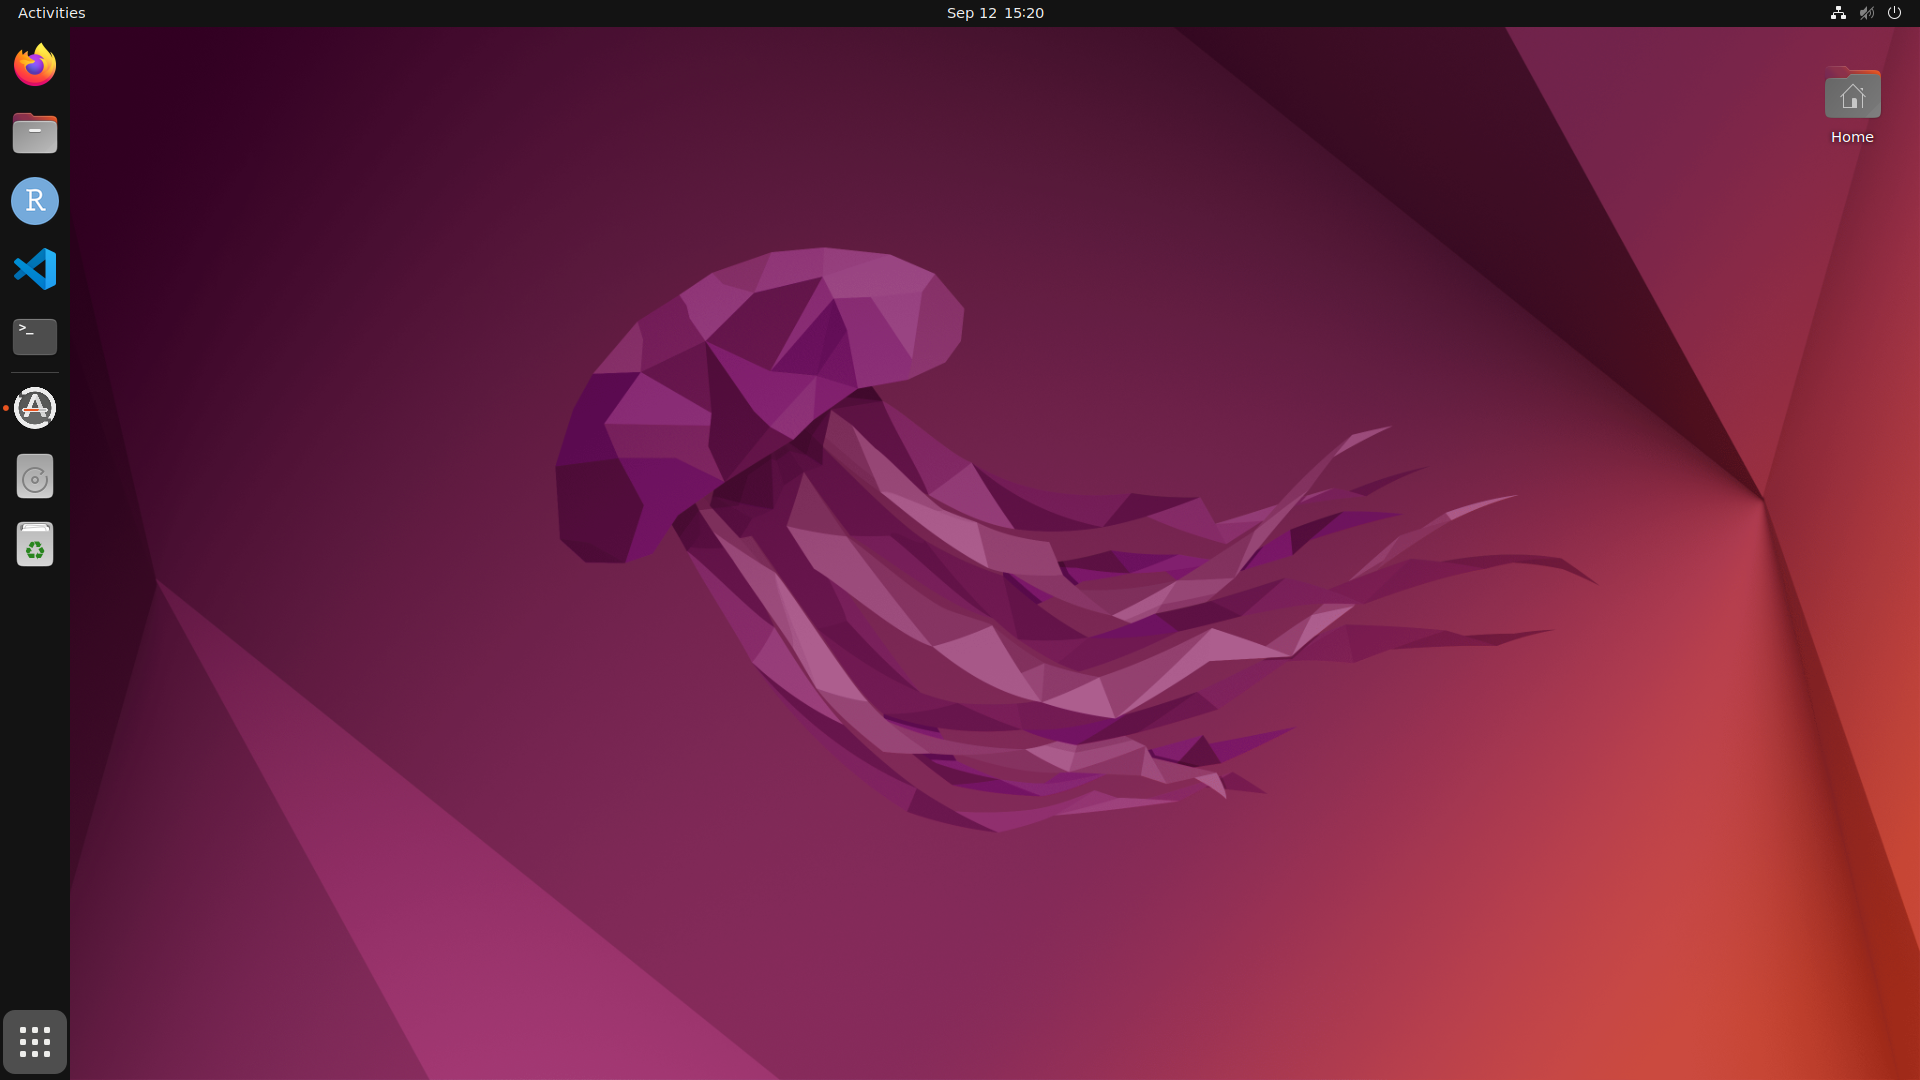
\includegraphics[width=15cm]{photos/Jammy.png}
\caption{Jammy Jellyfish}
\label{fig:figure1}
\end{figure}


\begin{equation}
    \text{NPP} = \text{GPP} - R_a
\end{equation}
\label{eq:NPP}
\myequations{NPP}



\begin{table}[h!]
\centering
\begin{tabular}{||c c||} 
 \hline
 Common Name & Scientific Name \\ [0.5ex] 
 \hline\hline
 Pine & \textit{Pinus sp.} \\ 
 Sal & \textit{Shorea robusta} \\
 ... & ... \\ [1ex] 
 \hline
\end{tabular}
\caption{Tree Species}
\label{table:species}
\end{table}


%%%%%%%%%%%%%%%%%%%%%%%%%%%%%%%%%%%%%%%%%%%%%%%%%%%%%%%%%%%%%%%%%%%%%%%%%%%%%%%%%%%%%%%%%%%%%%%%%%%%%%%%%%
\chapter{Review of Literature}



%%%%%%%%%%%%%%%%%%%%%%%%%%%%%%%%%%%%%%%%%%%%%%%%%%%%%%%%%%%%%%%%%%%%%%%%%%%%%%%%%%%%%%%%%%%%%%%%%%%%%%%%%%
\chapter{Study Area}
\begin{figure}
\centering
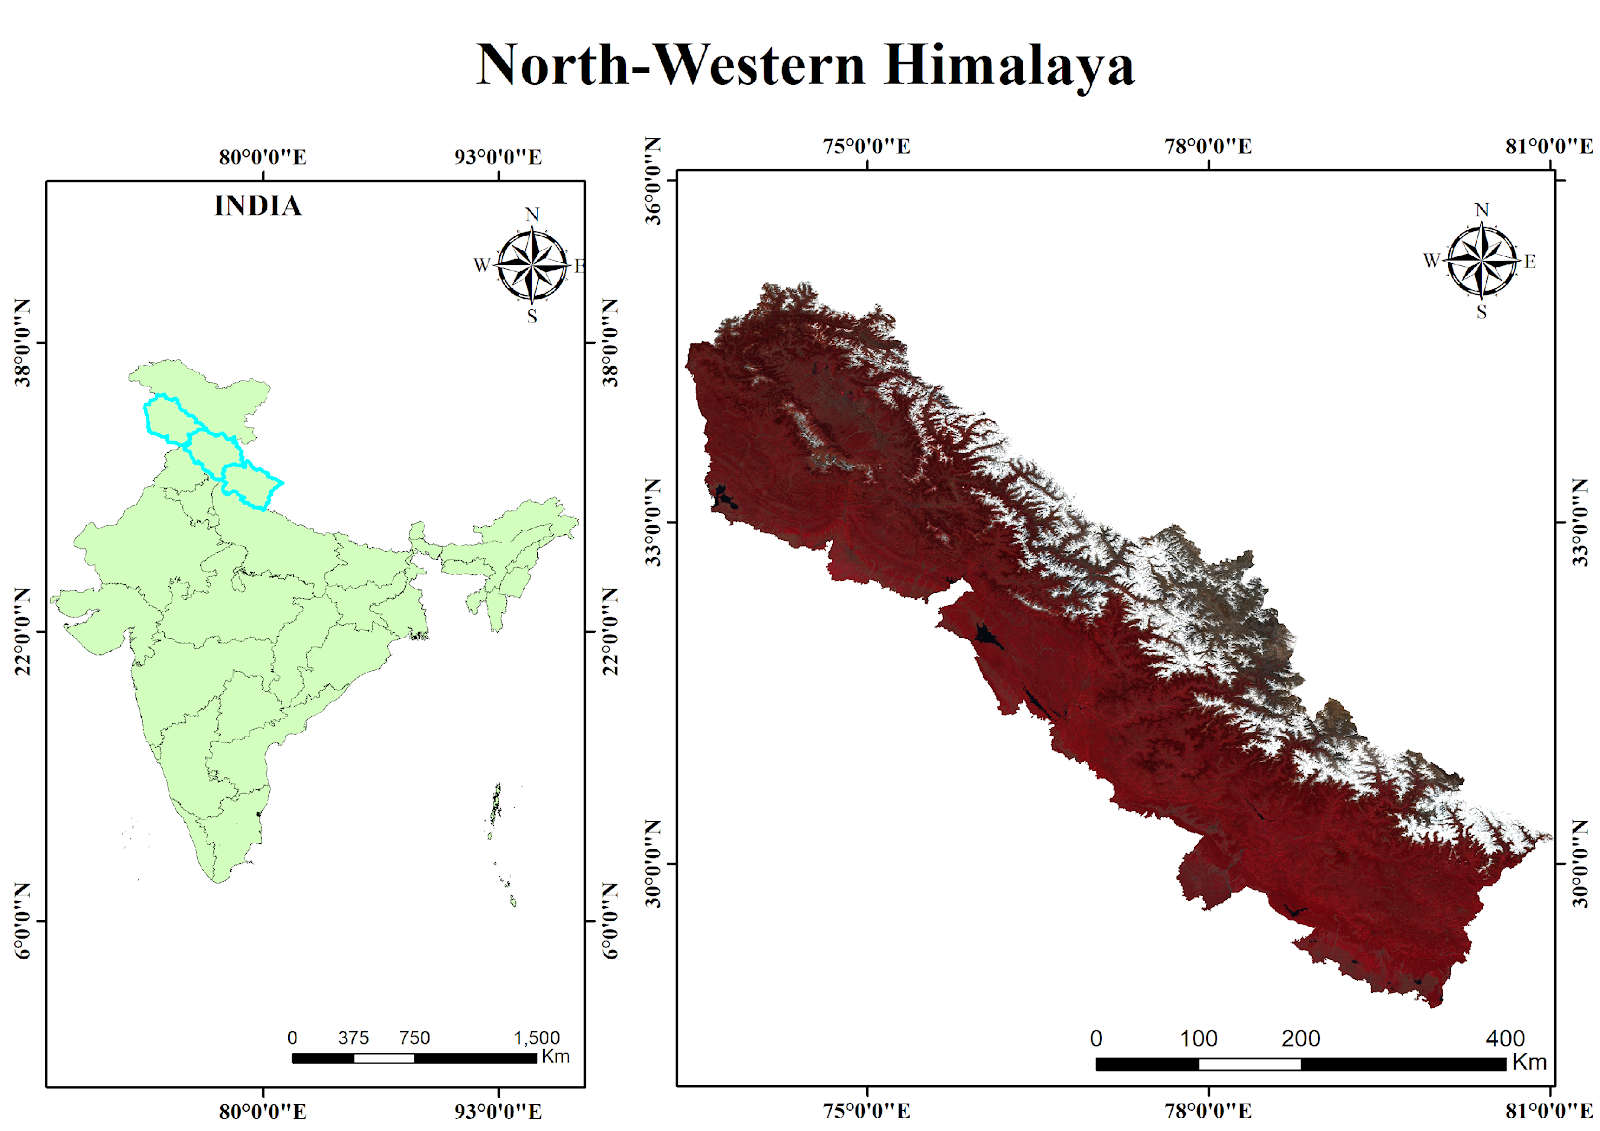
\includegraphics[width=15cm]{photos/NWH_Ph.png}
\caption{Study Area}
\label{fig: North Western Himalaya}
\end{figure}



 %%%%%%%%%%%%%%%%%%%%%%%%%%%%%%%%%%%%%%%%%%%%%%%%%%%%%%%%%%%%%%%%%%%%%%%%%%%%%%%%%%%%%%%%%%%%%%%%%%%%%%%%%%
 \chapter{Material and Method}
 
 
 %%%%%%%%%%%%%%%%%%%%%%%%%%%%%%%%%%%%%%%%%%%%%%%%%%%%%%%%%%%%%%%%%%%%%%%%%%%%%%%%%%%%%%%%%%%%%%%%%%%%%%%%%%

 \chapter{Result and Discussion}
 
 %%%%%%%%%%%%%%%%%%%%%%%%%%%%%%%%%%%%%%%%%%%%%%%%%%%%%%%%%%%%%%%%%%%%%%%%%%%%%%%%%%%%%%%%%%%%%%%%%%%%%%%%%%

 \chapter{Conclusion and Recommendation}
 

 %%%%%%%%%%%%%%%%%%%%%%%%%%%%%%%%%%%%%%%%%%%%%%%%%%%%%%%%%%%%%%%%%%%%%%%%%%%%%%%%%%%%%%%%%%%%%%%%%%%%%%%%%%

\newpage
\printbibliography

%%%%%%%%%%%%%%%%%%%%%%%%%%%%%%%%%%%%%%%%%%%%%%%%%%%%%%%%%%%%%%%%%%%%%%%%%%%%%%%%%%%%%%%%%%%%%%%%%%%%%%%%%%

% Adding vertical space before Appendix
\vspace*{2cm}
\newpage
%\phantomsection
%\addcontentsline{toc}{section}{APPENDIX}
\appendix

\chapter{Appendix I}
{\blindtext} %replace with actual appendix content

\chapter{Appendix II}
{blindtext} %  replace with actual appendix content


% Rest of your chapters go here
\end{document}
